The system recognizes two kind of gestures (see also
\ref{fig:gesturesToRecognize}):
\begin{itemize}
  \item A circle that starts from the bottom and runs clockwise
  \item A circle that starts from the bottom and runs counter-clockwise
\end{itemize}
The first gesture is used to mark an item as ``added to cart'' while the second
one serves to switch through the items on the shopping list.

\begin{figure}[h]
\captionsetup{justification=centering}
\begin{subfigure}{0.475\textwidth}
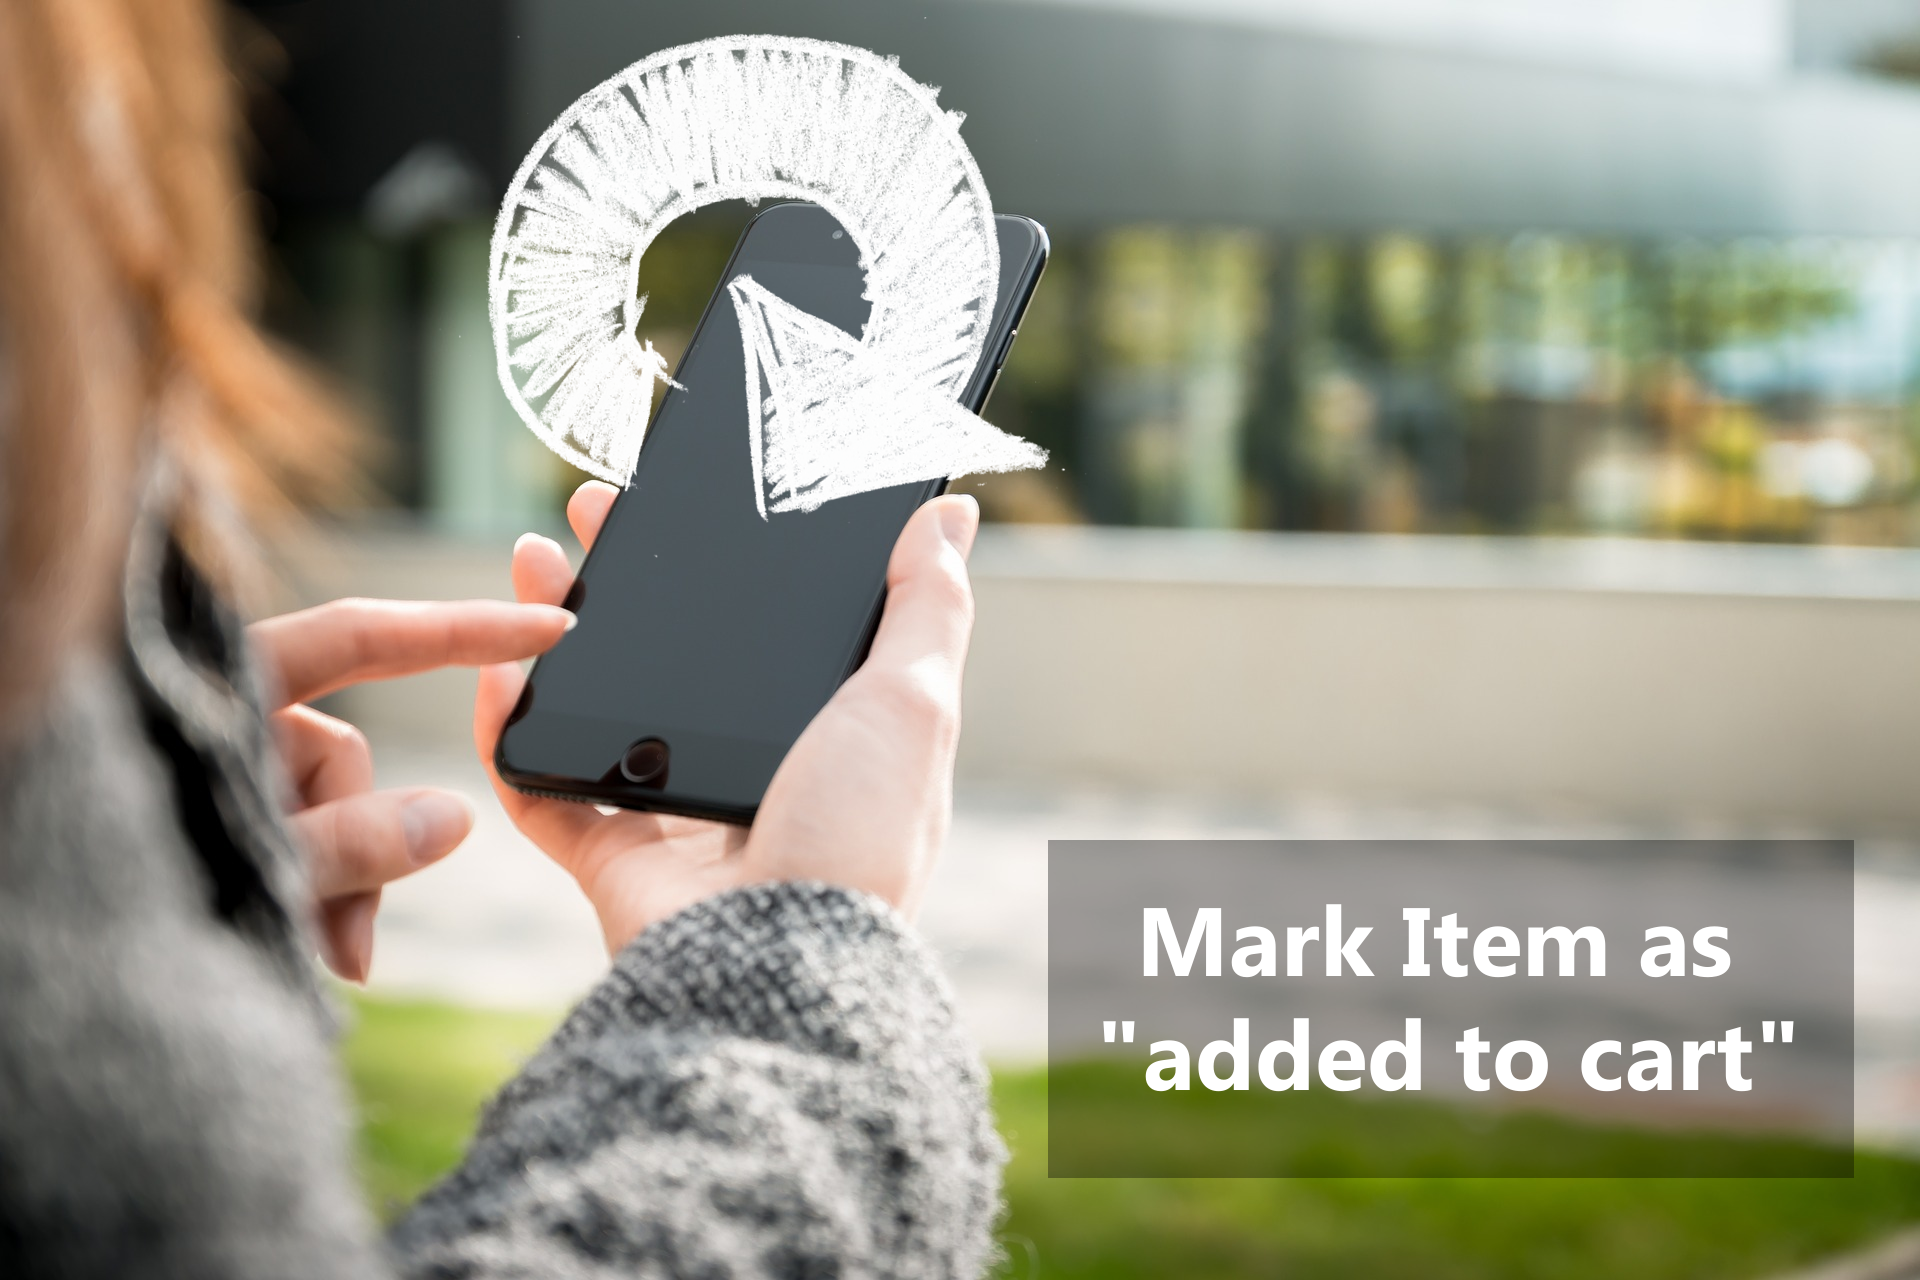
\includegraphics[width=\textwidth]{res/gestures/addToCart.png}
\caption{Add Item to Cart}
\label{fig:gestureAdd}
\end{subfigure} \hspace{0.05\textwidth}
\begin{subfigure}{0.475\textwidth}
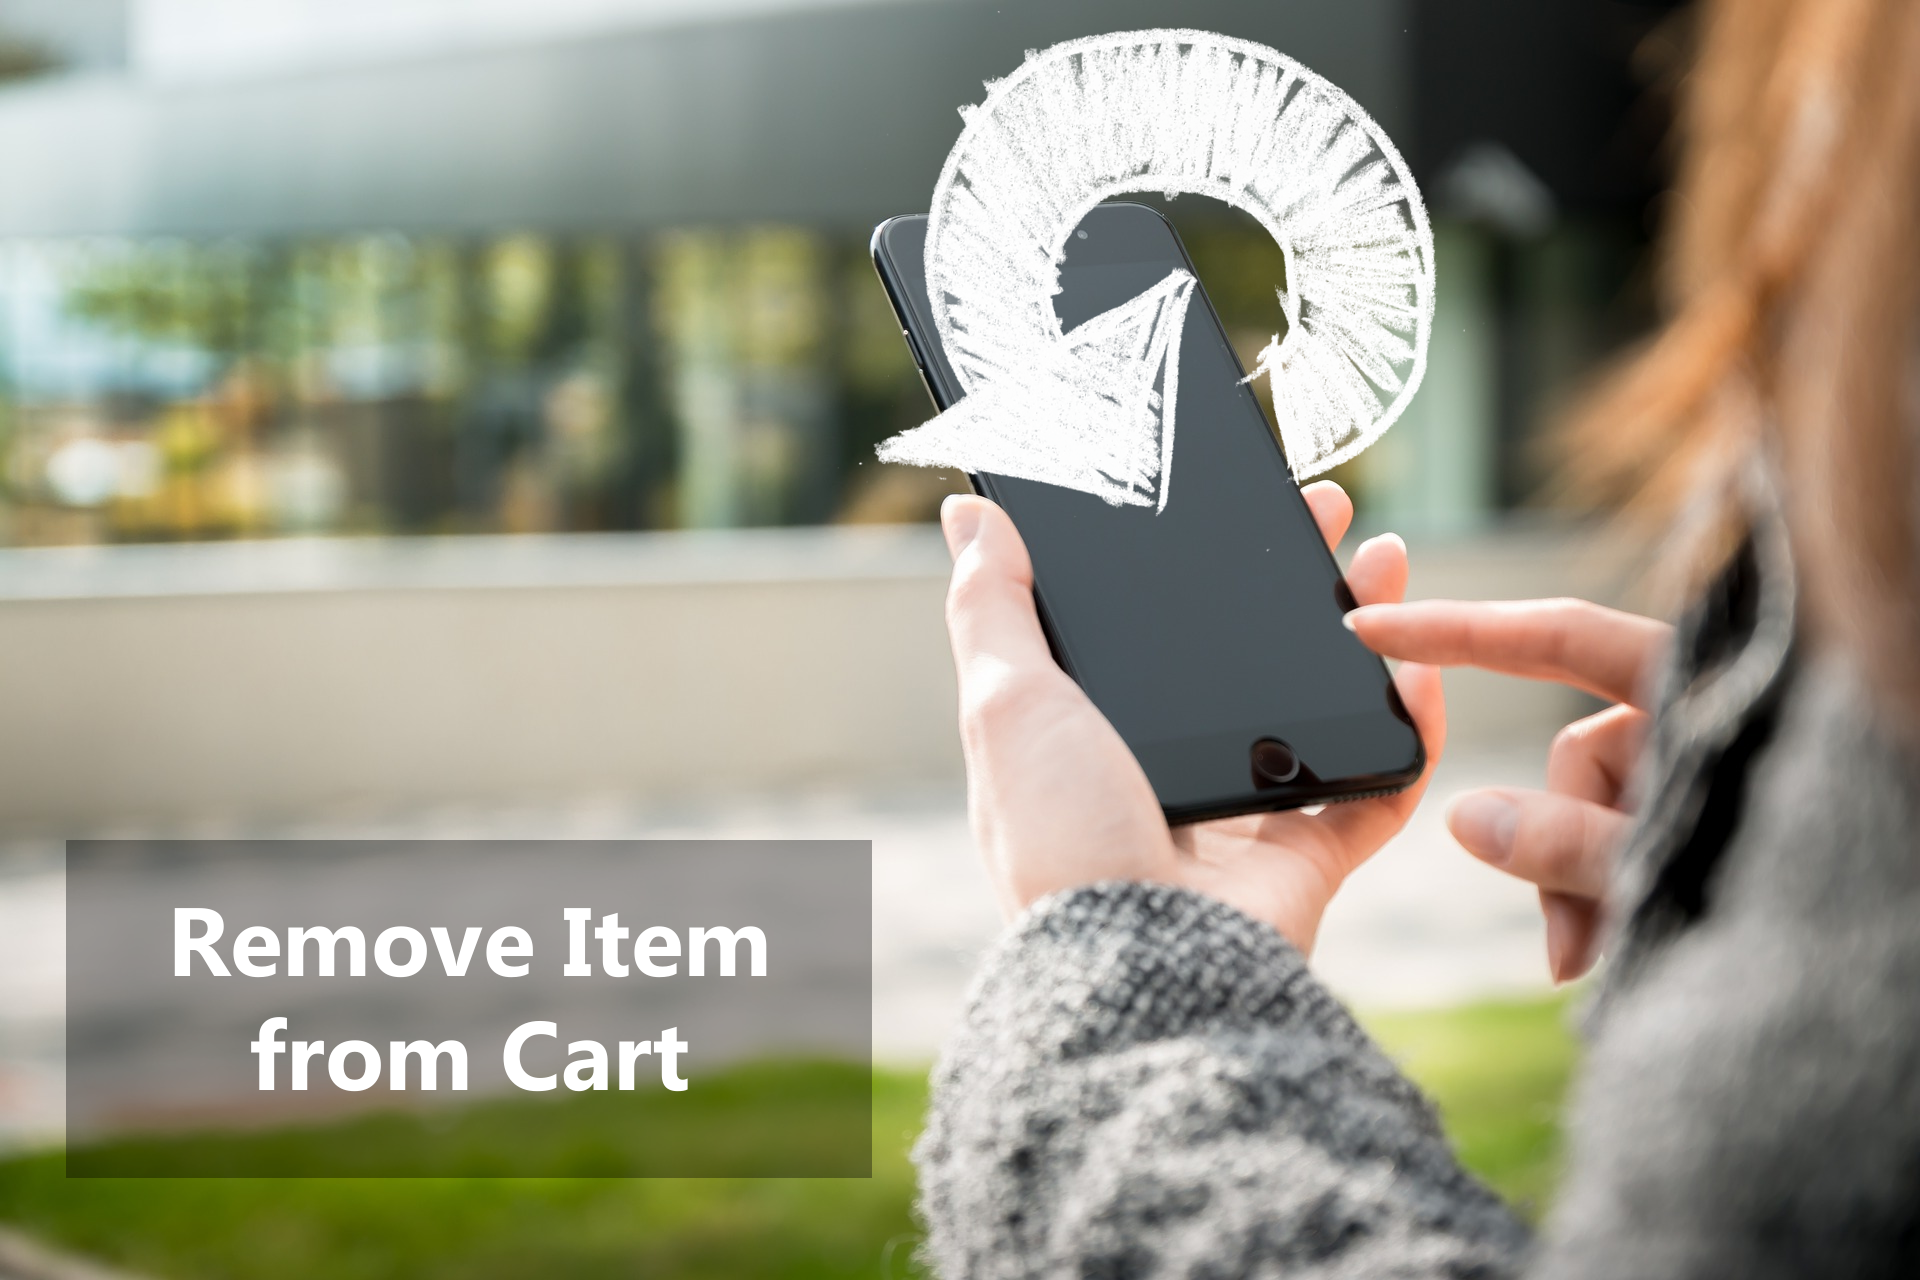
\includegraphics[width=\textwidth]{res/gestures/removeFromCart.png}
\caption{Switch Item}
\label{fig:gestureRemove}
\end{subfigure}
\caption{Gestures to Recognize}
\label{fig:gesturesToRecognize}
\end{figure}

\begin{figure}
\centering
\captionsetup{justification=centering}
\begin{tikzpicture}
\begin{axis}[
  id=Measured accelerations,
			width=0.9\textwidth,height=0.3\textheight,
			%title={Measured Accelerations},
    		grid =both,
    		minor x tick num = 1,
    		minor y tick num = 1,
			xlabel={Measurement Point},
			ylabel={Acceleration Values [$\frac{m}{s^2}$]}, ymin=-15, xmin=0,
			xmax=250, legend style={ at={(0,1)}, anchor=north west}]
\addplot [mark=none, blue, thick] 
		plot table [x=Point, y=a_{x}]{res/gestures/finalExcel.csv};
\addlegendentry{$a_x$}
\addplot [mark=none, ForestGreen, thick] 
		plot table [x=Point, y=a_{z}]{res/gestures/finalExcel.csv};
\addlegendentry{$a_z$}
\end{axis}
\end{tikzpicture}
\caption{Calculated Values $a_x$ and $a_z$ for two Circles}
\label{fig:finalAcc}
\end{figure}

\begin{figure}
\centering
\captionsetup{justification=centering}
\begin{tikzpicture}
\begin{axis}[
  id=Measured accelerations,
			width=0.9\textwidth,height=0.3\textheight,
			%title={Measured Accelerations},
    		grid =both,
    		minor x tick num = 1,
    		minor y tick num = 1,
			xlabel={Measurement Point},
			ylabel={Acceleration Values [$\frac{m}{s^2}$]}, ymin=-15, xmin=0,
			xmax=250, legend style={ at={(0,1)}, anchor=north west}] 
\addplot [mark=none, blue, thick] 
		plot table [x=Point, y=x]{res/gestures/kreis_flach_1.csv};
\addlegendentry{$a_x$}
\addplot [mark=none, magenta, thick] 
		plot table [x=Point, y=y]{res/gestures/kreis_flach_1.csv};
\addlegendentry{$a_y$}
\addplot [mark=none, ForestGreen, thick] 
		plot table [x=Point, y=z]{res/gestures/kreis_flach_1.csv};
\addlegendentry{$a_z$}
\end{axis}
\end{tikzpicture}
\caption{Calculated Values $a_x$ and $a_z$ for two Circles}
\label{fig:finalAcc}
\end{figure}
